\section{Background}
\label{sec:background}

\subsection{RDMA}

Remote Direct Memory Access, or RDMA, is a low-latency, high-throughput
networking technology which enables direct memory access (DMA) in the form of
read/write requests which bypass the CPU of the remote machine. 

For performance RDMA utilizes zero-copy from applications to the NIC which remove
the latency of copying data from user to kernel space with a CPU. This approach
bypasses the kernel which further reduces context switch latency.  Memory
accesses on a remote machine are managed entirely between the NIC and main
memory which eliminate all CPU and kernel induced overhead. These performance
enhancements allow RDMA to achieve $\mu$s-level latency and 100/200 Gbps
throughput in modern RDMA-enabled NICs (RNICs).

\subsection{RoCE and iWARP}

RDMA over Converged Ethernet (RoCE) is a popular implementation of RDMA. RoCE
was originally designed to run over InfiniBand network and uses
InfiniBand-specific headers for routing. 

RoCE in it's initial instantiation (RoCEV1) was a link later protocol. RoCEV1
packet headers are placed directly after an Ethernet header, see
~\ref{fig:roce_header_format}. RoCE practitioners craved routability and in it's
second incarnation RoCEV2 InfiniBand headers were placed after both an IP and
UDP header. RoCEV2 (sometimes referred to as routing RoCE (RRocE) increased the
protocols scope and scalability without considering the security implications of
enabling the protocol to route over the internet.

InfiniBand networks are designed to be lossless. To prevent RDMA packets from
being dropped or lost InfiniBand uses credit-based flow control to prioritize
RDMA payloads. By extension all RoCEV2 networks are expected to be lossless, a
single lost RDMA packet causes catastrophic performance degradation in RoCEV2.
To create the illusion of a lossless network outside of the InfiniBand
environment datacenter practitioners use the standardized 802.1 Qbb
Priority-based Flow Control, or PFC~\cite{802.1qbb}.

RoCE has comparable raw performance characteristics with RDMA on InfiniBand
network. It has made it possible to run RDMA in datacenters and it's gaining
popularity in recent years. Cloud operators like Microsoft Azure have started
providing RDMA-capable virtual machines~\cite{news:azure.rdma}.

\begin{figure*}[ht]
    \centering
    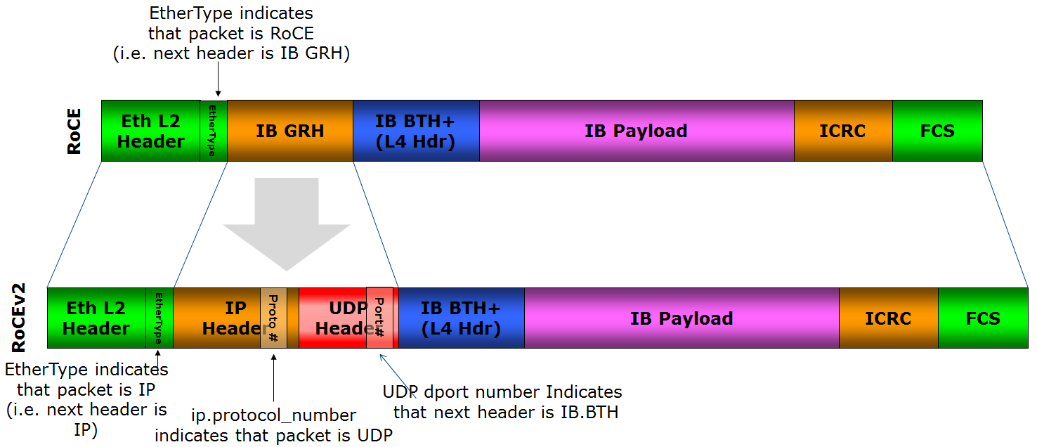
\includegraphics[width=\textwidth]{fig/RoCE_Header_format}
    \caption{RoCE v1 and RoCE v2 packet format}
    \label{fig:roce_header_format}
\end{figure*}

iWARP is an alliterative implementation of RDMA to RoCE. It drops the necessity of
a lossless networking, and instead sends RDMA packets over a traditional TCP
connection. While iWARP eliminates the need for hardware supported priority flow
control it takes a drastic hit in performance by incurring the latency of a TCP
stack. iWARPs poor performance in comparison to RoCE has lead to low adoption
among high performance application designers.

\subsection{RDMA Security}

RDMA protocol was originally designed to operate on High Performance
Computing (HPC) clusters.  

Such clusters are typically bespoke for a particular applications such as
large-scale physical simulations, and are isolated from other networks inside a
separated and trusted facility which have low security requirements.

The recent adoptions of RDMA in datacenters for cloud computing undermines the
assumption of separation and trust. Operating RDMA for cloud environment assumes
that malicious users might be able to perform side-channel attacks or even
compromise other virtual machines simply by colocation.  Concrete defense
measures need to be addressed to counter the emerging security issues from
datacenter-wide RDMA adoptions.
 
RDMA transfers data in raw bytes in favor of performance. This design decision
is only acceptable in the context of HPC clusters, not in a general datacenter .
Transferring encrypted data is an important but minimal requirement for securing
RDMA.  Protocol security is a holistic task encompassing every level of the
network stack. For instance both RoCE and iWARP could be made more secure via
existing tooling IPsec, and tcpcrypt respectively.  We argue for the end-to-end
principle and suggest that RDMA security should be TLS-like.  The inclusion of
encryption and authentication should only be on end hosts to prevent latency
incursion at intermediate switches and routers. DTLS is the counterpart of TLS
over UDP, and it works very similarly. Thus we only discuss a TLS-like
implementation for TCP in the following paragraphs.

The TLS protocol ensures three properties: secrecy, authenticity, and
reliability. Authenticity and reliability are less important in the datacenters.
Every computing instances in datacenters can be easily authenticated and we
assume the networking in datacenter is reliable as lossless. Secrecy can be hard
to achieve and we will present the difficulties at Sec.~\ref{sec:encrypt}. A TLS
implementation has two protocols: Handshake Protocols and Record Protocol. We
argue that only Record Protocol is required in datacenters because the handshake
protocols can be pre-assigned and updated in a fixed time period for a group of
known hosts. In a RoCEv2 packet, there are one 4-byte CRC checksum for Ethernet
FCS (Frame Check Sequence) and another 4-byye ICRC for RoCE v2 beyond Ethernet.
Using a 4-byte MAC is not enough for any secure MAC algorithm for today's
standard. For these reasons we argue that the MAC for TLS-enabled RDMA traffic
should be implemented in the payload of InfiniBand.

For RDMA, in a previous work, Security Enhancement in InfiniBand
Architecture~\cite{Lee:2005:SEI:1053727.1054449}, the paper achieves
authenticity by embedding an authentication tag in the header of an IBA packet.
\textcolor{red}{TBA}
